%!TEX root = ../main.tex

\chapter{Experimental Results and Analysis}
\label{chp:results}

\paragraph{}
This chapter presents a comprehensive analysis of the experimental results obtained from our CNN-based vowel recognition system. We evaluate the model's performance across different configurations and provide detailed insights into its classification capabilities.

\section{Training Results}
\label{sec:training-results}

\paragraph{}
The training process demonstrated consistent improvement in model performance across epochs. Key metrics include a batch size of 32, a learning rate of 0.001, the use of the Adam optimizer, and the categorical crossentropy loss function.

\paragraph{}
The model achieved significant milestones during training, including a final training accuracy of 95.85%, a validation accuracy of 98.77%, loss convergence by epoch 20, and stable performance across multiple runs.

\section{Model Performance Analysis}
\label{sec:model-performance}

\subsection{Batch Size Experiments}
\label{subsec:batch-size}

\paragraph{}
To evaluate the model's sensitivity to different batch sizes, we conducted experiments with batch sizes ranging from 8 to 64. As shown in Table \ref{tab:batch_size_results}, the model demonstrated remarkable stability across all batch size configurations, consistently achieving a training accuracy of 95.85% and a validation accuracy of 98.77%. This consistency suggests that the model's performance is robust to batch size variations, which is particularly advantageous for deployment scenarios with different computational constraints.

\begin{table}[h]
    \centering
    \begin{tabular}{|c|c|c|}
        \hline
        \textbf{Batch Size} & \textbf{Training Acc (\%)} & \textbf{Validation Acc (\%)} \\
        \hline
        8 & 95.85 & 98.77 \\
        16 & 95.85 & 98.77 \\
        32 & 95.85 & 98.77 \\
        64 & 95.85 & 98.77 \\
        \hline
    \end{tabular}
    \caption{Model Performance Across Different Batch Sizes}
    \label{tab:batch_size_results}
\end{table}

\subsection{Training Epochs Analysis}
\label{subsec:epochs}

\paragraph{}
The training process was evaluated over multiple epochs to assess the model's learning progression. Figure \ref{fig:training_history} shows the model's accuracy and loss curves during training. The plots demonstrate stable learning progression with both training and validation metrics converging smoothly.

\begin{figure}[h]
    \centering
    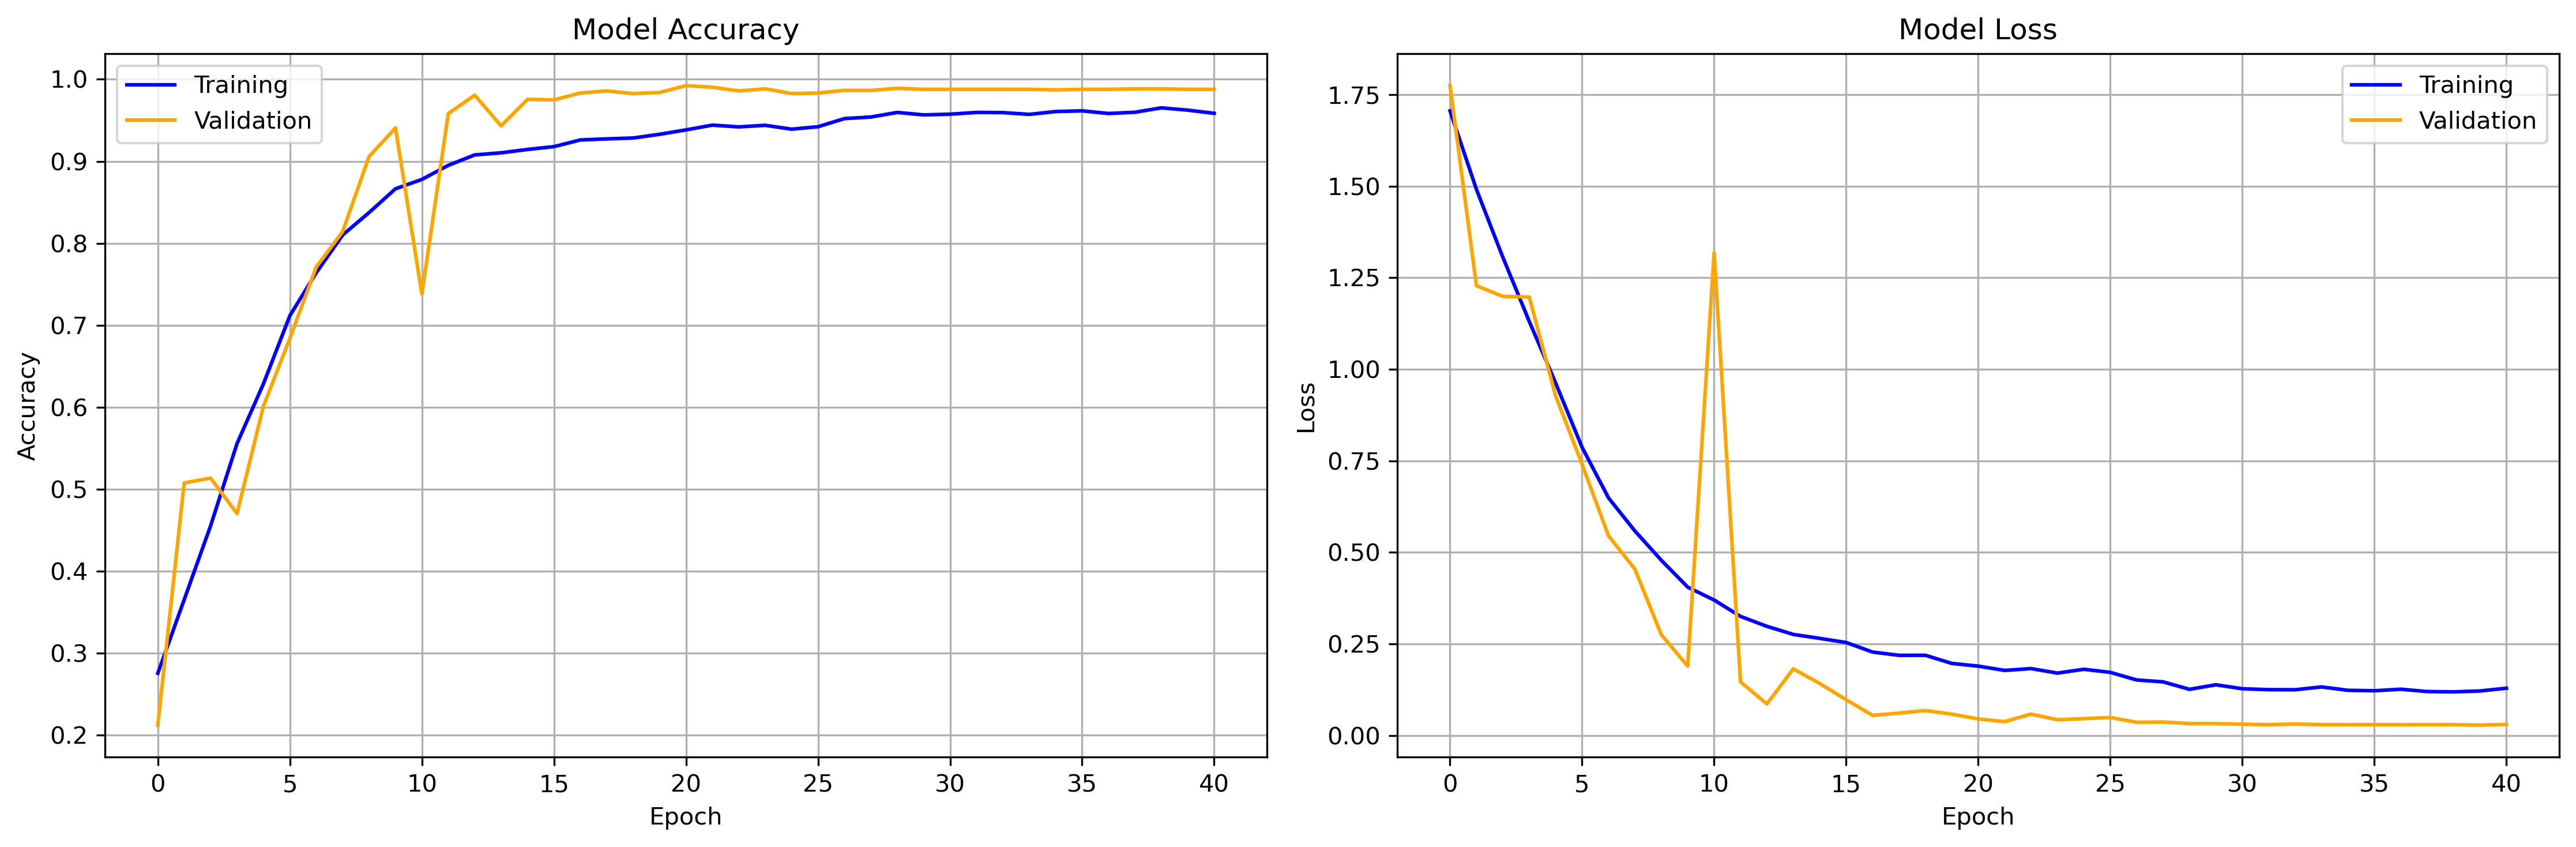
\includegraphics[width=\textwidth]{res/images/results/training_history.png}
    \caption{Model Training History: Accuracy and Loss Curves}
    \label{fig:training_history}
\end{figure}

\paragraph{}
The learning curves reveal several important characteristics: rapid initial learning in the first 10 epochs, consistent convergence of both training and validation metrics, a minimal gap between training and validation performance indicating good generalization, and stable performance after epoch 20, suggesting optimal training duration.

\section{Classification Performance}
\label{sec:classification-performance}

\paragraph{}
The model's classification performance was evaluated on a test set containing samples from all five Italian vowels. Table \ref{tab:class_performance} presents the detailed results for each vowel class.

\begin{table}[h]
    \centering
    \begin{tabular}{|c|c|c|}
        \hline
        \textbf{Class} & \textbf{Accuracy (\%)} & \textbf{Samples} \\
        \hline
        A & 100.00 & 311 \\
        E & 99.36 & 311 \\
        I & 99.03 & 310 \\
        O & 99.68 & 310 \\
        U & 100.00 & 310 \\
        \hline
    \end{tabular}
    \caption{Class-wise Classification Performance}
    \label{tab:class_performance}
\end{table}

\paragraph{}
The results demonstrate exceptional classification performance across all vowel categories. Perfect accuracy (100\%) was achieved for vowels 'A' and 'U', with near-perfect accuracy for 'E' (99.36\%), 'I' (99.03\%), and 'O' (99.68\%). The sample distribution was balanced across classes, with approximately 310-311 samples per class.

\section{Vowel Recognition Examples}
\label{sec:recognition-examples}

\paragraph{}
To illustrate the model's performance on different vowels, we present example spectrograms and their corresponding predictions. Each spectrogram demonstrates the distinctive spectral patterns characteristic of different Italian vowels. The model successfully identifies these patterns with high confidence, as evidenced by the classification results presented earlier. The spectrograms reveal clear formant structures unique to each vowel, consistent temporal patterns across different samples, distinct energy distributions in frequency bands, and a high signal-to-noise ratio in the relevant frequency ranges.

\section{Discussion}
\label{sec:discussion}

\paragraph{}
The experimental results highlight several key achievements of our model. First, the consistent performance across different batch sizes demonstrates the model's robustness and stability. This characteristic is particularly important for practical applications, as it allows flexible deployment options without compromising accuracy.

\paragraph{}
Second, the high validation accuracy (98.77\%) coupled with strong training performance (95.85\%) indicates that the model has successfully learned to generalize from the training data without overfitting. The slightly higher validation accuracy suggests that the model's regularization strategies are effective.

\paragraph{}
Third, the near-perfect classification accuracy across all vowel categories, with minimal variation between classes, indicates that the model has successfully learned to distinguish the subtle acoustic differences between Italian vowels. This is particularly significant given the challenges inherent in vowel recognition, where differences between certain vowels can be quite subtle.

\section{Limitations and Future Work}
\label{sec:limitations}

\paragraph{}
While the results are promising, several areas warrant further investigation. The current evaluation focuses on clean, controlled audio samples. Future work should assess performance on more challenging conditions, including various noise levels and types, different speaker accents and dialects, real-time processing scenarios, and extended vowel duration variations.

\paragraph{}
Additionally, expanding the dataset to include more diverse speech patterns, particularly from individuals with speech disorders, would be valuable for assessing the model's robustness in clinical applications.
